\documentclass[11pt,a4paper]{article}
\usepackage[margin=2.3cm]{geometry}
\usepackage{amsmath,amssymb}
\usepackage{graphicx}
\usepackage{booktabs}
\usepackage{multirow}
\usepackage{xcolor}
\usepackage[round,authoryear]{natbib}
\setcitestyle{aysep={,},yysep={,}}
\usepackage[colorlinks=true,linkcolor=blue!50!black,citecolor=blue!50!black,urlcolor=blue!50!black]{hyperref}
\urlstyle{same}
\usepackage{caption}
\captionsetup{font=small,labelfont=bf}
\graphicspath{{figures/}}
\DeclareMathOperator*{\argmin}{arg\,min}
\newcommand{\E}{\mathbb{E}}

\title{Playing osu! Like a Human:\\Cursor Generation with a TCN-WGAN and Key Press Decoding}
\author{pekin\\\small\url{https://github.com/pekingfather15/osuai}}
\date{October 2026}

\begin{document}
\maketitle

\begin{abstract}
We train neural networks to generate human-like play for the rhythm game osu! from recordings of human
players and play the generated data back in osu!lazer. The task is framed as imitation learning: the
models learn the conditional distribution of a player's cursor path and key presses given a map. Building
on the open-source project by niooii, we collect 1{,}992 replays and compare four established deep learning
sequence models (LSTM, VAE, WGAN-GP and a temporal convolutional WGAN) under one evaluation protocol. The
largest gains came from correcting training objectives rather than from new architectures. We show that
a finite-difference gradient penalty measures only about $1/\sqrt{d}=1/64$ of the critic's gradient,
that a squared-error loss provably drives the cursor to the spinner center, and that the evaluation used
half the real circle radius. With generator pretraining, a polar spinner head, a spin statistics loss and
a capped adversarial weight, the TCN-WGAN reaches 99.89\% Relax accuracy on 46 unseen maps (humans:
99.97\%) and spins at 396 RPM (humans: 371). For key presses, we find that near-simultaneous double presses
cause most of the accuracy lost in game; merging presses closer than 36\,ms, chosen on a validation set,
raises full accuracy from 93.55\% to 95.45\% (humans: 96.04\%). Playing logged out, the system scored
96.63\% on a 7.11-star map with Hidden and Hard Rock, with a hit-error UR of 81.
\end{abstract}

\section{Introduction}
osu! is a rhythm game in which the player moves a cursor onto circles, sliders and spinners and presses a
key in time with the music. It is also where the AI streamer Neuro-sama began: before it became a chatbot
VTuber, it was a program that played osu! \citep{neurosama}. That history is how this project began.

Writing a program that plays osu! perfectly is easy, since the map file specifies every object's position
and time. The harder and more interesting problem, shared with the project by \citet{niooii} on which this
work builds, is to make a program play \emph{like a human}, with smooth but imperfect cursor paths, real
spinning and natural key timing. This is a machine learning problem: there is no
formula for ``human-like'', so the behaviour has to be learned from examples of human play.

The work makes the following contributions:
\begin{itemize}
  \item a formulation of the task as conditional generative modelling for imitation learning, and an
        explanation, from this formulation, of why deterministic regressors such as LSTMs cannot spin;
  \item a data pipeline and fixed test/validation splits over 1{,}992 replays, with held-out maps
        identified by the hash of the map file;
  \item an evaluation that scores generated and human plays identically, validated against in-game results;
  \item a diagnosis of why the original GAN models did not aim or spin, with fixes that make the
        TCN-WGAN the best model;
  \item an analysis of key press errors in game and a decoding step that removes most of them;
  \item playback in osu!lazer, the current open-source client \citep{lazer}, restricted to logged-out play.
\end{itemize}

\section{Background}
\subsection{The game}
A map is a sequence of hit objects, each with a position on a $512\times384$ playfield and a time. Circles
must be clicked on time, sliders must be clicked and then followed while a key is held, and spinners must
be spun around the centre. The circle radius is $r = 54.4-4.48\,\mathrm{CS}$ osu!pixels, where CS is the
map's circle size \citep{wikics}. The hit windows depend on the overall difficulty (OD): a press within
$80-6\,\mathrm{OD}$\,ms of the object's time scores 300, within $140-8\,\mathrm{OD}$\,ms 100, and within
$200-10\,\mathrm{OD}$\,ms 50 \citep{wikiod}. At OD 10 a player must press within $\pm20$\,ms for a 300.
Accuracy is
\begin{equation}
  \mathrm{acc}=\frac{300\,n_{300}+100\,n_{100}+50\,n_{50}}{300\,(n_{300}+n_{100}+n_{50}+n_{\mathrm{miss}})}.
  \label{eq:acc}
\end{equation}
Players describe timing consistency with the unstable rate (UR), ten times the standard deviation of the
hit errors in milliseconds. The Relax mod presses keys automatically, so an accuracy measured with Relax
reflects only the cursor.

\subsection{Human movement}
Two classic results describe what human cursor movement looks like. Fitts' law states that the time to
reach a target grows with $\log_2(2D/W)$, where $D$ is the distance and $W$ the target width
\citep{fitts1954}, so humans slow down for far or small targets. The minimum-jerk model shows that point-to-point
arm movements follow the smoothest path, minimising the integral of the squared jerk (the derivative of
acceleration), which yields smooth, bell-shaped velocity profiles \citep{flash1985}. Human movement is also
variable: no two players, and no two attempts by one player, produce the same path. A human-like model must
therefore produce smooth paths and a \emph{distribution} of paths rather than a single answer.

\subsection{Learning from demonstrations}
Learning a behaviour from recordings of an expert is called imitation learning; its simplest form,
behavioural cloning, treats it as supervised learning from observations to actions \citep{pomerleau1989,
hussein2017}. Here the observation is the map $x$ (a sequence of features per time step) and the action is
the player's cursor path and key state $y$. A known weakness of behavioural cloning is covariate shift:
when the agent's own mistakes lead it to states the expert never visited, errors compound \citep{ross2011}.
Our setting avoids this, because generation is open-loop: the whole play is generated from the map before
the game starts, and the game state does not feed back into the model.

What a model can learn depends on its loss. A model trained with the squared error learns the
conditional mean:
\begin{equation}
  \argmin_f \E\left[\lVert y-f(x)\rVert^2\right] = \E[y \mid x]
  \label{eq:mean}
\end{equation}
\citep[Section 1.5.5]{bishop2006}. When $p(y\mid x)$ has a single mode, the mean is a good answer, which is
why regressors aim well. When it has many modes, the mean can be an answer no human would give. On a
spinner, players draw circles of different phases around the centre; averaging over the phase $\phi$,
$\E_\phi[c + r(\cos\phi,\sin\phi)] = c$, the centre itself. A deterministic regressor therefore sits still
on spinners. To be human-like a model has to \emph{sample} from $p(y\mid x)$, which is what generative models do.

\section{Models}
All models are deep neural networks trained by gradient descent. Section~\ref{sec:frontier} compares them
with current models.

\subsection{Recurrent networks and LSTM}
A recurrent network reads a sequence one step at a time and keeps a hidden state $h_t$ that summarises the
past. Plain recurrent networks are hard to train over long sequences because gradients shrink or explode as
they are propagated back through many steps. The long short-term memory (LSTM) adds a cell state $c_t$ that
is updated additively and controlled by gates \citep{hochreiter1997, gers2000}:
\begin{align}
  i_t,\,f_t,\,o_t &= \sigma\left(W\,[h_{t-1},x_t] + b\right), \qquad
  \tilde c_t = \tanh\left(W_c\,[h_{t-1},x_t] + b_c\right),\\
  c_t &= f_t\odot c_{t-1} + i_t\odot \tilde c_t, \qquad h_t = o_t\odot\tanh(c_t),
\end{align}
where the input, forget and output gates $i_t, f_t, o_t$ decide what is written, kept and read. LSTMs have
generated human handwriting from pen trajectories \citep{graves2013}, a task close to ours. Trained with a
squared error (or the Huber loss used here, which is quadratic for small errors), however, an LSTM is a
regressor and outputs the mean path of Eq.~\eqref{eq:mean}.

\subsection{Temporal convolutional networks}
A temporal convolutional network (TCN) replaces recurrence with stacked one-dimensional convolutions. A
causal convolution only uses inputs up to time $t$; a dilated convolution with kernel size $k$ and dilation
$d$ looks at inputs $t, t-d, \dots, t-(k-1)d$ \citep{yu2016, oord2016}. Doubling the dilation in each layer
grows the receptive field exponentially with depth:
\begin{equation}
  R = 1 + (k-1)\sum_{\ell=1}^{L} d_\ell, \qquad d_\ell = 2^{\ell-1}.
\end{equation}
TCNs process all time steps in parallel and have been found to match or outperform LSTMs on many sequence
tasks while keeping a longer effective memory \citep{bai2018}. Because the whole map is known in advance, we
can also shift some layers to look into the future. Convolutions also support the second-order gradients
that the gradient penalty needs, which an LSTM in cuDNN does not (Section 5.1).

\subsection{Variational autoencoders}
A variational autoencoder (VAE) learns a latent variable model $p_\theta(y\mid z,x)$ with a prior $p(z)$.
Since the likelihood cannot be computed directly, an encoder $q_\phi(z\mid y,x)$ approximates the posterior,
and both are trained to maximise the evidence lower bound \citep{kingma2014vae, rezende2014}:
\begin{equation}
  \log p_\theta(y\mid x) \ge \E_{q_\phi(z\mid y,x)}\left[\log p_\theta(y\mid z,x)\right]
  - \mathrm{KL}\left(q_\phi(z\mid y,x)\,\Vert\,p(z)\right).
\end{equation}
Sampling $z$ gives different outputs for the same map. With a powerful decoder, however, the model can
ignore $z$ and drive the KL term to zero; this \emph{posterior collapse} \citep{bowman2016} turns the VAE back
into a mean predictor. Adversarial VAEs add a discriminator to improve realism \citep{plumerault2020}.

\subsection{Generative adversarial networks and WGAN-GP}
A generative adversarial network (GAN) trains a generator $G(z,x)$ against a discriminator that tries to tell
real data from generated data \citep{goodfellow2014}; conditioning both on $x$ gives a conditional GAN
\citep{mirza2014}. The original objective is unstable and prone to mode collapse, in which the generator
covers only a few modes. The Wasserstein GAN instead minimises the earth mover's distance, which by the
Kantorovich--Rubinstein duality is
\begin{equation}
  W(p_r,p_g)=\sup_{\lVert D\rVert_L\le 1}\;\E_{y\sim p_r}[D(y)]-\E_{y\sim p_g}[D(y)],
\end{equation}
where the critic $D$ must be 1-Lipschitz \citep{arjovsky2017}. WGAN-GP enforces this with a gradient penalty
on random interpolates $\hat y$ between real and generated samples \citep{gulrajani2017}:
\begin{equation}
  \mathcal{L}_{\mathrm{GP}} = \lambda\,\E_{\hat y}\left[\left(\lVert\nabla_{\hat y} D(\hat y)\rVert_2-1\right)^2\right].
  \label{eq:gp}
\end{equation}
Computing $\nabla_\theta\mathcal{L}_{\mathrm{GP}}$ requires differentiating a gradient (double backpropagation).
Adversarial losses are often combined with a reconstruction loss that keeps outputs close to the target,
as in image-to-image translation \citep{isola2017}; we do the same.

\subsection{Relation to the state of the art}
\label{sec:frontier}
None of these architectures is new: LSTM dates from 1997, VAE and GAN from 2014, WGAN-GP from 2017 and the
TCN as evaluated here from 2018. They are established methods, chosen because they fit a dataset of
10{,}730 training segments and one laptop GPU, and because the original project implemented them. The state
of the art in sequence and motion generation has since moved to Transformers \citep{vaswani2017},
denoising diffusion models \citep{ho2020}, which generate human body motion with high realism
\citep{tevet2023}, and state-space models such as Mamba \citep{gu2023}. These models are larger and more data
hungry. This work does not propose a new architecture. It analyses why the established ones failed on this
task and fixes them using the principles above.

\subsection{Related work on osu!}
OsuLearn trained a recurrent network on replays to generate cursor movement \citep{osulearn}.
\citet{niooii} extended it with a VAE, a WGAN-GP with an LSTM critic and a TCN-WGAN, reporting Relax
accuracies of 98.10\% (LSTM), 98.89\% (VAE), 99.68\% (LSTM-WGAN) and 99.40\% (TCN-WGAN) on one map in a video.
The author notes that the LSTM is ``too good'' and robotic, that the VAE averages movement and cannot reliably
spin, and that the TCN variant ``is probably not set up well''. Keys come from a separate LSTM that
``sometimes will tap twice for trickier sequences''; this paper finds that this double tapping is the main
source of lost accuracy in game. Other open-source projects generate cursor movement for an editor
\citep{osucad} or play from screen captures with object detection \citep{autosu}.

\section{Data}
\paragraph{Sources.} Replays of the players ranked first and third in the world were downloaded from the
official website (671 replays). To cover more players we imported the osu!3k dataset \citep{osu3k} (MIT
licence), selecting replays by player performance points with accuracy $\ge 90\%$ and star rating $\ge 5$,
and excluding mods that change the game (Relax, Autopilot, Spun Out, Easy, Half Time). Maps were downloaded
from a mirror and matched to replays by the MD5 hash of the map file.

\paragraph{Cleaning.} Some osu!3k entries are the same play rendered twice with different mods; all such
conflicting duplicates were dropped. 20 replays by players with under 2{,}000 total pp but high-star,
high-accuracy scores were excluded as implausible.

\paragraph{Splits.} The test set holds 50 replays (46 usable) downloaded after V1 was trained, on maps never
used for training, one replay per map. A validation set of 30 replays (27 usable) is used only to choose
checkpoints and decoding settings. From V3 on, test and validation maps are excluded by file hash rather than
path, which caught 9 more replays of the same maps stored in other folders.

\paragraph{Representation.} Each map becomes a sequence of 12\,ms frames with 9 features: the position of the
next object, the time until it, the object type, CS, and slider speed and length. The target is the cursor
position and the state of the two keys. Sequences are cut into chunks of 2{,}048 frames (24.6\,s).

\begin{table}[t]
\centering
\caption{Dataset versions. A segment is 2{,}048 frames of 12\,ms.}
\label{tab:data}
\begin{tabular}{lll}
\toprule
Version & Training replays & Segments \\
\midrule
V1 & 212 (two players) & 1{,}409 \\
V2 & 425 (two players) & 2{,}530 \\
V3 & 1{,}992 (official 671 + osu!3k 1{,}410; over 1{,}000 players) & 10{,}730 \\
\midrule
\citet{niooii} & -- & 13{,}617 \\
\bottomrule
\end{tabular}
\end{table}

\section{Method}
\subsection{TCN-WGAN cursor model}
The generator is a TCN with kernel size 3 over the map features concatenated with an 8-dimensional noise
sequence. Its first six layers (dilations 1 to 32) each shift the kernel two frames into the future, so the
generator sees 12 frames (144\,ms) ahead, and its last four layers are causal; in total it sees 1.7\,s of the past. The critic is a TCN over the map features and a cursor trajectory whose seven dilated layers each look
one frame ahead, and outputs one score per sequence. The
generator has 277{,}956 parameters, the critic 141{,}025. The generator loss is
\begin{equation}
  \mathcal{L}_G = \mathcal{L}_{\mathrm{pos}} - \lambda_{\mathrm{adv}}\,\E[D(G(z,x),x)] + \lambda_{\mathrm{spin}}\,\mathcal{L}_{\mathrm{spin}},
\end{equation}
where $\mathcal{L}_{\mathrm{pos}}$ is the Huber (smooth L1) position error, which is quadratic for errors
below 1 and therefore behaves like the squared error of Eq.~\eqref{eq:mean} when aiming. The critic uses the
exact penalty of
Eq.~\eqref{eq:gp} with $\lambda=8$ and three critic steps per generator step. We use Adam
\citep{kingma2015} with $\beta=(0.5,0.9)$.

\paragraph{Why the original penalty did not work.} The original WGAN code replaced Eq.~\eqref{eq:gp} with a
finite difference along one random unit direction $u$, $(D(\hat y+\epsilon u)-D(\hat y))/\epsilon \approx
u^\top g$ with $g=\nabla D(\hat y)$, to avoid double backpropagation through the LSTM critic. For $u$ uniform
on the unit sphere in $\mathbb{R}^d$, $\E[(u^\top g)^2]=\lVert g\rVert^2/d$, so $|u^\top g|\approx\lVert
g\rVert/\sqrt d$. A trajectory of 2{,}048 frames with $(x,y)$ has $d=4{,}096$ dimensions, so the penalty sees
only $1/64$ of the gradient and pushes $\lVert g\rVert$ towards 64 instead of 1. The critic is then far from
1-Lipschitz; in our runs its loss stalled near 3.66 and the Wasserstein estimate stayed near 0, meaning it
could not separate real from generated play. The exact penalty with an LSTM critic took 12.2\,s per step
(cuDNN's LSTM does not support double backward) against 0.13\,s for the approximation, which is impractical;
a convolutional critic computes it cheaply, which is why we use the TCN.

\paragraph{Pretraining.} The original learning rate of $10^{-4}$ was still reducing the position error after
100 epochs. We first train the generator for 60 epochs on $\mathcal{L}_{\mathrm{pos}}$ alone at $10^{-3}$,
then train adversarially at $10^{-4}$, ramping $\lambda_{\mathrm{adv}}$ up to at most $2\times10^{-4}$. A
larger weight let the critic's scores grow and pulled the cursor away from the targets.

\paragraph{Spinners.} Following Eq.~\eqref{eq:mean}, a position loss on spinner frames pulls the cursor to the
centre, so we remove spinner frames from $\mathcal{L}_{\mathrm{pos}}$. A separate polar head outputs a radius
$r_t$ and an angular speed $\omega_t$ during spinners:
\begin{equation}
  (x_t,y_t)=c+r_t\,(\cos\theta_t,\sin\theta_t),\qquad \theta_t=\theta_0+s\sum_{\tau\le t}\omega_\tau,
\end{equation}
where $c$ is the playfield centre and the start angle $\theta_0$ and direction $s\in\{-1,1\}$ come from the
noise. Separating the head keeps spinner training from interfering with aiming. The spin statistics loss asks
for at least the players' mean angular speed $\bar\omega$ and a similar mean radius $\bar r$, but not for a
particular phase, so it has no averaging problem:
\begin{equation}
  \mathcal{L}_{\mathrm{spin}}=\max(0,\bar\omega_{\mathrm{real}}-\bar\omega_{\mathrm{fake}})
  +\left(\frac{\bar r_{\mathrm{fake}}-\bar r_{\mathrm{real}}}{100}\right)^2,
\end{equation}
with $\lambda_{\mathrm{spin}}=0.02$ from epoch 30.

\subsection{Key model and decoding}
Keys come from the original key model: a two-layer LSTM (64 units) and a dense layer that predict, for each
frame, the probability that each of the two keys is held (54{,}626 parameters), trained with binary
cross-entropy against the human key state. Two properties of this formulation explain its errors. First, a
press lasts one frame while a hold lasts five to ten, so the loss is dominated by hold frames and barely
changes when the press moment is off by a frame; press events are rare, a class imbalance familiar from
object detection \citep{lin2017}. Second, the model is often unsure which key a human would use, so both
probabilities hover near 0.5 and thresholding each key separately presses both within a frame or two
(Fig.~\ref{fig:keys}). In game every extra press can hit the next object early, and in osu!lazer only the key
that hit a slider head keeps tracking the slider, so a short extra press that reaches the head first and lets
go loses the slider tail.

We therefore decode presses: presses that start less than $g$ apart are merged into one, held until the last
of them is released, and each press gets a key that is not already held, releasing a key for one frame before
pressing it again. Merging near-duplicate detections is the idea behind non-maximum suppression in object
detection \citep{neubeck2006}. The gap $g$ is chosen on the validation set.

\begin{figure}[t]
\centering
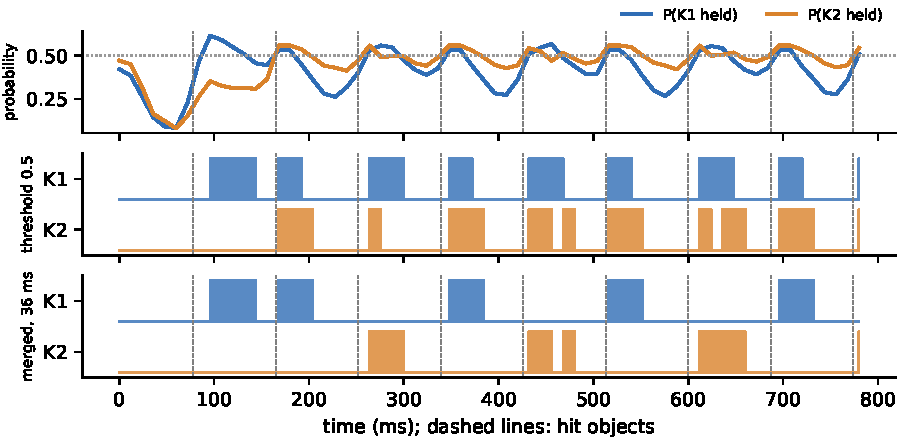
\includegraphics[width=\linewidth]{key_decoding.pdf}
\caption{Key model output in an 800\,ms stream on a 7.88-star map. Top: hold probabilities. Middle:
thresholding each key at 0.5 presses both keys at almost every object. Bottom: after merging presses closer
than 36\,ms. Presses also come slightly after the objects (7\,ms on average over the map), a delay the
playback offset compensates.}
\label{fig:keys}
\end{figure}

\subsection{Playback in osu!lazer}
The original playback reads osu!stable's memory. For osu!lazer we read the game state from the websocket of
tosu \citep{tosu}: the map file, the song time, the mods and the profile. The song time arrives every
10--20\,ms, so it is extrapolated with the local clock between updates and never allowed to step back by less
than 50\,ms. The cursor is mapped to the screen with lazer's playfield transform (scale $h/480$, centred). Key
changes of skipped frames are replayed in order, and an offset compensates for the playback latency. A small
window generates the play when a map is selected, can generate the cursor alone for testing with the Relax
mod, and enables playback only when tosu reports that nobody is logged in.

\subsection{Implementation}
The V3 models were trained with the project's first implementation, which was built on the code of
\citet{niooii}. All code in the repository was then rewritten for this project: map and replay parsing
(including the slider curves, which now follow the curve types of the .osu format instead of a coarse
approximation), the features, the models, training, evaluation and playback. The V3 weights were converted to
the new code and give identical outputs for identical inputs. The results of Sections 7.1 and 7.2 come from
the first implementation; the key decoding results and Table~\ref{tab:keys} were recomputed with the new code.

\section{Evaluation}
For every test replay the model generates a play for the same map and mods, and the generated and human plays
are scored the same way:
\begin{itemize}
  \item \textbf{Relax accuracy}: each circle or slider head is judged by the closest moment within its 50
        window at which the cursor is inside the circle, as if the game pressed the keys.
  \item \textbf{Full accuracy}: judged with the key presses. Each press of either key can hit one object; an
        object takes the earliest unused press in its window while the cursor is inside.
  \item \textbf{Slider tails}: the key that hit the head must stay held, and the cursor inside the follow
        circle ($2.4r$), until 36\,ms before the slider ends.
  \item \textbf{Spinner RPM}: rotations around the playfield centre during spinners.
\end{itemize}
The original evaluation code used half the real circle radius; all numbers here use the corrected radius
unless stated. Full accuracy underestimates real accuracy: the human replays score 95.84\% here but 99.00\%
according to the replay files, mostly because 12\,ms sampling loses some short presses. The evaluation is
nevertheless predictive: for the 7.88-star map below it predicts 90.63\% and 391/420 slider tails, and the
game reported 90.09\% and 393/420. The rewritten evaluation reproduces the first one: on the same 46 test
plays the V3 TCN-WGAN scores 93.44\% full accuracy without and 95.47\% with press merging (first
implementation: 93.41\% and 95.49\%), with identical Relax accuracy (99.89\%), hit rate, mean distance and
spinner speed. It can also read 4 test maps the first parser could not, so the tables below use all 50.

\section{Results}
\subsection{Cursor models}
Table~\ref{tab:main} compares all models on the 46 test maps with the same key model, and
Fig.~\ref{fig:traj} shows their trajectories.

\begin{table}[t]
\centering
\caption{Test set (46 unseen maps), first implementation, corrected radius, all with the V3 key model (no
decoding, first version of the full-accuracy judge).}
\label{tab:main}
\small
\begin{tabular}{lrrrrr}
\toprule
Source & Full acc. & Relax acc. & Relax misses & Mean dist. & Spinner \\
\midrule
Human & 95.84\% & 99.97\% & 5 & 11.9\,px & 371 RPM \\
V1 LSTM & 94.94\% & 99.95\% & 14 & 9.1\,px & 3 \\
V1 WGAN-GP & 62.53\% & 80.49\% & 4{,}988 & 33.7\,px & 41 \\
V2 LSTM & 94.79\% & 99.96\% & 13 & 9.7\,px & 6 \\
V2 VAE & 51.92\% & 71.13\% & 8{,}219 & 39.1\,px & 42 \\
V2 WGAN-GP & 81.55\% & 91.95\% & 2{,}482 & 24.3\,px & 34 \\
V2 TCN-WGAN (original settings) & 73.19\% & 91.17\% & 1{,}962 & 26.3\,px & 29 \\
V3 LSTM & 94.76\% & 99.92\% & 27 & 10.6\,px & 3 \\
\textbf{V3 TCN-WGAN} & \textbf{94.68\%} & \textbf{99.89\%} & \textbf{28} & \textbf{8.3\,px} & \textbf{396} \\
\bottomrule
\end{tabular}
\end{table}

\begin{figure}[t]
\centering
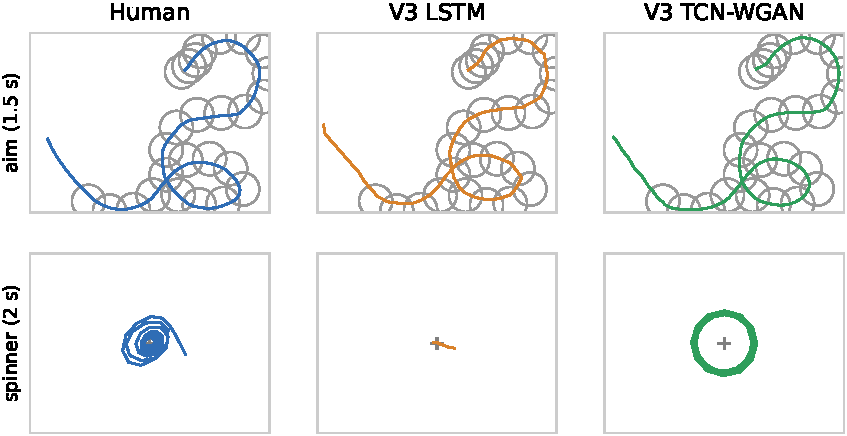
\includegraphics[width=0.92\linewidth]{trajectories.pdf}
\caption{Cursor paths on an unseen map. Top: 1.5\,s of aiming. Bottom: the first 2\,s of a spinner. The LSTM
aims as well as the GAN but stays at the spinner centre, as Eq.~\eqref{eq:mean} predicts.}
\label{fig:traj}
\end{figure}

The results follow the principles of Section 2. The LSTMs aim almost perfectly, as expected from a regressor
on a single-mode target, but never spin (3--6 RPM). The VAE's KL term fell to near zero in every version, a
posterior collapse that leaves it a mean predictor, and its spinner loss is again a position loss. The
original GAN models aim poorly, which we trace to the penalty and the learning rate. After the fixes the V3
TCN-WGAN aims as precisely as the LSTM and spins like a human. More diverse data (V3, over a thousand players)
made the LSTM slightly worse, as its mean path becomes an average of more styles, but helped the GAN, which
samples from the distribution of styles.

\subsection{Ablation}
Table~\ref{tab:ablation} adds the fixes one at a time on V2 data. These numbers use the old, halved radius and
are only comparable with each other.

\begin{table}[t]
\centering
\caption{Ablation of the TCN-WGAN on V2 data (test set, old halved radius).}
\label{tab:ablation}
\begin{tabular}{lrrr}
\toprule
Change & Relax acc. & Mean dist. & Spinner \\
\midrule
Original settings (100 epochs, lr $10^{-4}$) & 56.5\% & 26.6\,px & 24 RPM \\
+ generator pretraining (40 epochs, lr $10^{-3}$) & 96.7\% & 10.1\,px & 26 \\
+ no position loss on spinners, spin loss (shared output) & 89.9\% & 14.7\,px & 86 \\
+ polar spinner head & 89.3\% & 14.5\,px & 372 \\
+ 60 pretraining epochs, $\lambda_{\mathrm{adv}}\le 2\times10^{-4}$ & 97.4\% & 9.5\,px & 519 \\
\bottomrule
\end{tabular}
\end{table}

\begin{figure}[t]
\centering
\begin{minipage}{0.48\linewidth}
\centering
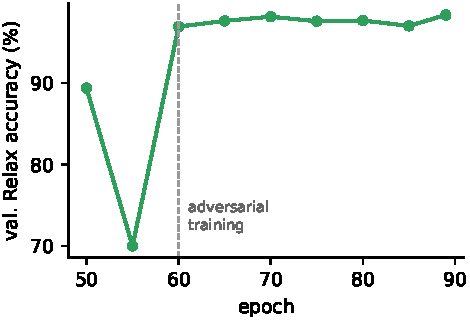
\includegraphics[width=\linewidth]{checkpoints.pdf}
\caption{V3 TCN-WGAN checkpoints on the validation set (old radius). Epoch 89 was chosen.}
\label{fig:ckpt}
\end{minipage}\hfill
\begin{minipage}{0.48\linewidth}
\centering
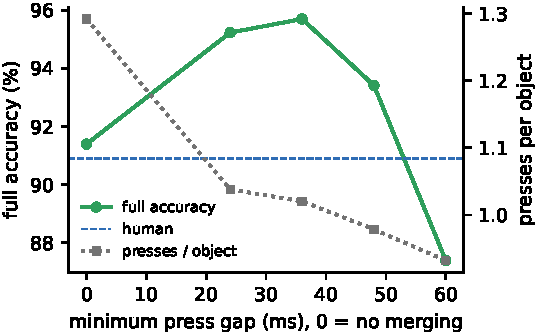
\includegraphics[width=\linewidth]{gap_sweep.pdf}
\caption{Choosing the press merging gap on the validation set.}
\label{fig:gap}
\end{minipage}
\end{figure}

Pretraining alone raised Relax accuracy from 56.5\% to 96.7\%. Sharing the output between aiming and spinning
cost accuracy, which the separate polar head and the lower adversarial weight recovered. Accuracy varies a lot
between checkpoints (70\% at epoch 55, 97\% at epoch 60; Fig.~\ref{fig:ckpt}), as is common in adversarial
training, so checkpoints must be chosen on a validation set.

\subsection{Key decoding}
The judge was updated to count each key's presses separately and to score slider tails. Fig.~\ref{fig:gap}
and Table~\ref{tab:keys} show that merging presses closer than 36\,ms brings the presses per object from 1.29
to 1.02 (humans: 1.00) and full accuracy above the human replays on the validation set. Larger gaps start
merging real presses in fast streams.

\begin{table}[t]
\centering
\caption{Key decoding, V3 TCN-WGAN with the V3 key model, scored with the rewritten evaluation
(30 validation and 50 test plays).}
\label{tab:keys}
\small
\begin{tabular}{llrrrr}
\toprule
Set & Decoding & Full acc. & 300/100/50/miss & Slider tails & Presses/obj. \\
\midrule
\multirow{4}{*}{Validation} & human & 90.89\% & 20906/1482/31/1131 & 94.3\% & 1.00 \\
 & threshold 0.5 & 91.39\% & 20856/1555/890/249 & 94.5\% & 1.29 \\
 & merged, 24\,ms & 95.23\% & 22097/881/215/357 & 96.4\% & 1.04 \\
 & merged, 36\,ms & 95.70\% & 22270/739/124/417 & 96.4\% & 1.02 \\
\midrule
\multirow{3}{*}{Test} & human & 96.04\% & 37150/2244/31/40 & 99.4\% & 1.03 \\
 & threshold 0.5 & 93.55\% & 36052/2108/982/323 & 95.3\% & 1.16 \\
 & \textbf{merged, 36\,ms} & \textbf{95.45\%} & 37259/1031/405/770 & 95.8\% & 1.00 \\
\bottomrule
\end{tabular}
\end{table}

Merging removes most 50s but adds misses (323 to 770 on the test set): some real presses are merged away.
The V3 LSTM, scored the same way, reaches 95.74\% with merging; its keys come from the same key model, and it
aims slightly more precisely, but it does not spin (3 RPM).
Decoding cannot fully fix a model that was trained to predict held states rather than press events.

\section{In-Game Results}
All runs were played in osu!lazer while logged out (guest), full screen at $1920\times1080$, with the V3
TCN-WGAN and the V3 key model (Table~\ref{tab:ingame}). Hit errors were recorded from tosu
(Fig.~\ref{fig:hits}).

\begin{table}[t]
\centering
\caption{In-game results in osu!lazer (guest). Maps by Ado (first three) and Kenshi Yonezu. Offset: playback
latency compensation in ms; merged: presses closer than 36\,ms merged. Offline: prediction of the evaluation
for the same map.}
\label{tab:ingame}
\small
\begin{tabular}{lrlrrl}
\toprule
Map & Stars & Settings & Accuracy & 300/100/50/miss & Offline \\
\midrule
AiAiA [Kiss me Insane] & 4.07 & offset 15 & 98.38\% & 668/12/2/3 & -- \\
AiAiA [Be loved Expert] & 5.70 & offset 15 & 95.85\% & 820/39/15/3 & 97.30\%$^\dagger$ \\
Aishite Aishite Aishite [$<$/3] & 7.88 & offset 15 & 74.88\% & 579/394/40/21 & -- \\
\quad same map & 7.88 & offset 29 & 90.09\% & 876/69/68/21 & 90.63\% \\
IRIS OUT [Darling!!!] & 7.11 & HD HR, 29, merged & \textbf{96.63\%} & 654/28/0/5 & 97.96\% \\
\bottomrule
\end{tabular}

\raggedright\footnotesize $^\dagger$ first version of the judge.
\end{table}

\begin{figure}[t]
\centering
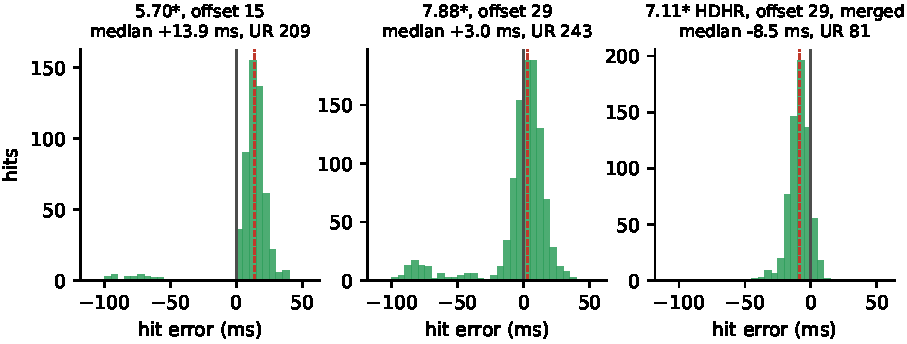
\includegraphics[width=\linewidth]{hit_errors.pdf}
\caption{Hit errors recorded in game (positive = late). Left: presses about 14\,ms late before calibrating the
offset. Middle: centred, but with a tail of presses 60--100\,ms early (one beat early at 230 BPM). Right:
after merging the tail is gone and UR is 81.}
\label{fig:hits}
\end{figure}

The first run on the 7.88-star map (OD 9.6, $\pm22$\,ms for a 300) lost most 300s to a systematic delay of
about 14\,ms. Offline, adding a 7\,ms delay and 15\,ms jitter to the presses reproduced the game result almost
exactly (73.80\%, 646/328/42/17), which shows how sensitive a narrow window is to timing noise. Calibrating the
offset raised it to 90.09\%. The remaining 50s and the 27 lost slider tails came from double presses:
simulating the game's rules offline lost exactly 27 tails. After merging, the 7.11-star map with Hard Rock
(OD 10, $\pm20$\,ms) scored 96.63\% without a single 50, with a hit-error standard deviation of 8.1\,ms
(UR 81), against a UR of 209 and 243 in the two earlier recorded runs.

\section{Discussion}
\paragraph{Lessons.}
(1) An approximation of a training objective can silently break the method: the finite-difference penalty
measured $1/\sqrt d$ of the gradient, and the critic never learned. (2) An optimiser setting can matter more
than the architecture: pretraining at a higher learning rate turned 56.5\% into 96.7\%. (3) The loss decides
what the model can represent: a squared error cannot produce a multi-modal behaviour such as spinning, and the
VAE's spinner loss had the same flaw. (4) Too much adversarial weight trades accuracy for realism. (5) For
keys, predicting held states per frame makes the press moment unimportant to the loss and invites double
presses. (6) The evaluation must match the game: a halved radius and a judge that merged the two keys hid
real problems, and once corrected, offline predictions matched the game within about one percentage point.

\paragraph{Limitations.}
The full-accuracy judge underestimates humans and does not model note lock or slider ticks. Human-likeness is
argued from trajectories and statistics (spinner speed, presses per object, UR), not measured with a
perceptual study. The playback latency drifts by about 10\,ms between sessions. Merging adds misses. Only five
in-game runs were recorded. V3 still has 79\% of the original author's data.

\paragraph{Future work.}
A key model that predicts press events with a sub-frame offset, with a focal or weighted loss for the rare
events \citep{lin2017}, a release tied to the end of the object it hit, a non-causal TCN, and the generated
cursor as input, should remove double presses without merging away real ones. A single model for cursor and
keys would let presses depend on where the cursor is. Diffusion models \citep{ho2020, tevet2023} are the
natural next step for the cursor model if more data becomes available.

\section{Ethics}
All in-game experiments were played while logged out of osu!, so nothing was submitted to the online
leaderboards; using such playback on an online account breaks the game's rules and is unfair to other
players. The playback has no anti-detection features. Music and map files are not redistributed. The osu!3k
dataset is used under its MIT licence.

\section*{Acknowledgements}
Thanks to niooii for the original project and models, to GuiBrandt for OsuLearn, to the authors of osu!3k, and
to the developers of tosu and osu!lazer. The code, experiments and this paper were developed with the help of
Claude (Anthropic) as a coding assistant. The code is available at
\url{https://github.com/pekingfather15/osuai}.

\newpage
\renewcommand{\refname}{References}
% Reference list in APA 7th style, shared by paper_en.tex and paper_zh.tex
\begingroup
\setlength{\bibsep}{4pt}
\setlength{\bibhang}{0.5in}
\small
\begin{thebibliography}{99}

\bibitem[{Arjovsky et~al.}(2017)]{arjovsky2017}
Arjovsky, M., Chintala, S., \& Bottou, L. (2017). Wasserstein generative adversarial networks. In D.~Precup \&
Y.~W. Teh (Eds.), \emph{Proceedings of the 34th International Conference on Machine Learning} (Vol.~70,
pp.~214--223). PMLR. \url{https://proceedings.mlr.press/v70/arjovsky17a.html}

\bibitem[{Bai et~al.}(2018)]{bai2018}
Bai, S., Kolter, J.~Z., \& Koltun, V. (2018). \emph{An empirical evaluation of generic convolutional and
recurrent networks for sequence modeling} [Preprint]. arXiv. \url{https://doi.org/10.48550/arXiv.1803.01271}

\bibitem[{Bishop}(2006)]{bishop2006}
Bishop, C.~M. (2006). \emph{Pattern recognition and machine learning}. Springer.

\bibitem[{Bowman et~al.}(2016)]{bowman2016}
Bowman, S.~R., Vilnis, L., Vinyals, O., Dai, A.~M., Jozefowicz, R., \& Bengio, S. (2016). Generating sentences
from a continuous space. In \emph{Proceedings of the 20th SIGNLL Conference on Computational Natural Language
Learning} (pp.~10--21). Association for Computational Linguistics. \url{https://doi.org/10.18653/v1/K16-1002}

\bibitem[{Fitts}(1954)]{fitts1954}
Fitts, P.~M. (1954). The information capacity of the human motor system in controlling the amplitude of
movement. \emph{Journal of Experimental Psychology, 47}(6), 381--391. \url{https://doi.org/10.1037/h0055392}

\bibitem[{Flash \& Hogan}(1985)]{flash1985}
Flash, T., \& Hogan, N. (1985). The coordination of arm movements: An experimentally confirmed mathematical
model. \emph{The Journal of Neuroscience, 5}(7), 1688--1703.
\url{https://doi.org/10.1523/JNEUROSCI.05-07-01688.1985}

\bibitem[{gameswu}(n.d.)]{autosu}
gameswu. (n.d.). \emph{AutOsu} [Computer software]. GitHub. Retrieved October 7, 2026, from
\url{https://github.com/gameswu/AutOsu}

\bibitem[{Gers et~al.}(2000)]{gers2000}
Gers, F.~A., Schmidhuber, J., \& Cummins, F. (2000). Learning to forget: Continual prediction with LSTM.
\emph{Neural Computation, 12}(10), 2451--2471. \url{https://doi.org/10.1162/089976600300015015}

\bibitem[{Goodfellow et~al.}(2014)]{goodfellow2014}
Goodfellow, I., Pouget-Abadie, J., Mirza, M., Xu, B., Warde-Farley, D., Ozair, S., Courville, A., \& Bengio, Y.
(2014). Generative adversarial nets. In \emph{Advances in Neural Information Processing Systems} (Vol.~27).
Curran Associates.

\bibitem[{Graves}(2013)]{graves2013}
Graves, A. (2013). \emph{Generating sequences with recurrent neural networks} [Preprint]. arXiv.
\url{https://doi.org/10.48550/arXiv.1308.0850}

\bibitem[{Gu \& Dao}(2023)]{gu2023}
Gu, A., \& Dao, T. (2023). \emph{Mamba: Linear-time sequence modeling with selective state spaces} [Preprint].
arXiv. \url{https://doi.org/10.48550/arXiv.2312.00752}

\bibitem[{GuiBrandt}(n.d.)]{osulearn}
GuiBrandt. (n.d.). \emph{OsuLearn} [Computer software]. GitHub. Retrieved October 7, 2026, from
\url{https://github.com/GuiBrandt/OsuLearn}

\bibitem[{Gulrajani et~al.}(2017)]{gulrajani2017}
Gulrajani, I., Ahmed, F., Arjovsky, M., Dumoulin, V., \& Courville, A.~C. (2017). Improved training of
Wasserstein GANs. In \emph{Advances in Neural Information Processing Systems} (Vol.~30). Curran Associates.

\bibitem[{Ho et~al.}(2020)]{ho2020}
Ho, J., Jain, A., \& Abbeel, P. (2020). Denoising diffusion probabilistic models. In \emph{Advances in Neural
Information Processing Systems} (Vol.~33, pp.~6840--6851). Curran Associates.

\bibitem[{Hochreiter \& Schmidhuber}(1997)]{hochreiter1997}
Hochreiter, S., \& Schmidhuber, J. (1997). Long short-term memory. \emph{Neural Computation, 9}(8), 1735--1780.
\url{https://doi.org/10.1162/neco.1997.9.8.1735}

\bibitem[{Hussein et~al.}(2017)]{hussein2017}
Hussein, A., Gaber, M.~M., Elyan, E., \& Jayne, C. (2017). Imitation learning: A survey of learning methods.
\emph{ACM Computing Surveys, 50}(2), Article 21. \url{https://doi.org/10.1145/3054912}

\bibitem[{ilymeow}(n.d.)]{osu3k}
ilymeow. (n.d.). \emph{osu!3k} [Data set]. Kaggle. Retrieved October 7, 2026, from
\url{https://www.kaggle.com/datasets/ilymeow/osu3k}

\bibitem[{Isola et~al.}(2017)]{isola2017}
Isola, P., Zhu, J.-Y., Zhou, T., \& Efros, A.~A. (2017). Image-to-image translation with conditional adversarial
networks. In \emph{Proceedings of the IEEE Conference on Computer Vision and Pattern Recognition}
(pp.~1125--1134). IEEE. \url{https://doi.org/10.1109/CVPR.2017.632}

\bibitem[{Kingma \& Ba}(2015)]{kingma2015}
Kingma, D.~P., \& Ba, J. (2015). Adam: A method for stochastic optimization. In \emph{3rd International
Conference on Learning Representations}. \url{https://doi.org/10.48550/arXiv.1412.6980}

\bibitem[{Kingma \& Welling}(2014)]{kingma2014vae}
Kingma, D.~P., \& Welling, M. (2014). Auto-encoding variational Bayes. In \emph{2nd International Conference on
Learning Representations}. \url{https://doi.org/10.48550/arXiv.1312.6114}

\bibitem[{Lin et~al.}(2017)]{lin2017}
Lin, T.-Y., Goyal, P., Girshick, R., He, K., \& Doll\'ar, P. (2017). Focal loss for dense object detection. In
\emph{Proceedings of the IEEE International Conference on Computer Vision} (pp.~2980--2988). IEEE.
\url{https://doi.org/10.1109/ICCV.2017.324}

\bibitem[{minetoblend}(n.d.)]{osucad}
minetoblend. (n.d.). \emph{osucad-cursor-predict} [Computer software]. GitHub. Retrieved October 7, 2026, from
\url{https://github.com/minetoblend/osucad-cursor-predict}

\bibitem[{Mirza \& Osindero}(2014)]{mirza2014}
Mirza, M., \& Osindero, S. (2014). \emph{Conditional generative adversarial nets} [Preprint]. arXiv.
\url{https://doi.org/10.48550/arXiv.1411.1784}

\bibitem[{Neubeck \& Van~Gool}(2006)]{neubeck2006}
Neubeck, A., \& Van Gool, L. (2006). Efficient non-maximum suppression. In \emph{18th International Conference
on Pattern Recognition} (Vol.~3, pp.~850--855). IEEE. \url{https://doi.org/10.1109/ICPR.2006.479}

\bibitem[{Neuro-sama}(n.d.)]{neurosama}
Neuro-sama. (n.d.). In \emph{Wikipedia}. Retrieved October 7, 2026, from
\url{https://en.wikipedia.org/wiki/Neuro-sama}

\bibitem[{niooii}(2026)]{niooii}
niooii. (2026). \emph{osu} [Computer software]. GitHub. \url{https://github.com/niooii/osu}

\bibitem[{Plumerault et~al.}(2020)]{plumerault2020}
Plumerault, A., Le Borgne, H., \& Hudelot, C. (2020). \emph{AVAE: Adversarial variational auto encoder}
[Preprint]. arXiv. \url{https://doi.org/10.48550/arXiv.2012.11551}

\bibitem[{Pomerleau}(1989)]{pomerleau1989}
Pomerleau, D.~A. (1989). ALVINN: An autonomous land vehicle in a neural network. In D.~S. Touretzky (Ed.),
\emph{Advances in Neural Information Processing Systems} (Vol.~1, pp.~305--313). Morgan Kaufmann.

\bibitem[{ppy}(n.d.-a)]{lazer}
ppy. (n.d.-a). \emph{osu!} [Computer software]. GitHub. Retrieved October 7, 2026, from
\url{https://github.com/ppy/osu}

\bibitem[{ppy}(n.d.-b)]{wikics}
ppy. (n.d.-b). Circle size. In \emph{osu! wiki}. Retrieved October 7, 2026, from
\url{https://osu.ppy.sh/wiki/Beatmap/Circle_size}

\bibitem[{ppy}(n.d.-c)]{wikiod}
ppy. (n.d.-c). Overall difficulty. In \emph{osu! wiki}. Retrieved October 7, 2026, from
\url{https://osu.ppy.sh/wiki/Beatmap/Overall_difficulty}

\bibitem[{Rezende et~al.}(2014)]{rezende2014}
Rezende, D.~J., Mohamed, S., \& Wierstra, D. (2014). Stochastic backpropagation and approximate inference in deep
generative models. In \emph{Proceedings of the 31st International Conference on Machine Learning} (Vol.~32,
pp.~1278--1286). PMLR.

\bibitem[{Ross et~al.}(2011)]{ross2011}
Ross, S., Gordon, G., \& Bagnell, D. (2011). A reduction of imitation learning and structured prediction to
no-regret online learning. In \emph{Proceedings of the Fourteenth International Conference on Artificial
Intelligence and Statistics} (Vol.~15, pp.~627--635). PMLR.

\bibitem[{Tevet et~al.}(2023)]{tevet2023}
Tevet, G., Raab, S., Gordon, B., Shafir, Y., Cohen-Or, D., \& Bermano, A.~H. (2023). Human motion diffusion
model. In \emph{The Eleventh International Conference on Learning Representations}.
\url{https://doi.org/10.48550/arXiv.2209.14916}

\bibitem[{tosu}(n.d.)]{tosu}
tosu. (n.d.). \emph{tosu} [Computer software]. GitHub. Retrieved October 7, 2026, from
\url{https://github.com/tosuapp/tosu}

\bibitem[{van~den Oord et~al.}(2016)]{oord2016}
van den Oord, A., Dieleman, S., Zen, H., Simonyan, K., Vinyals, O., Graves, A., Kalchbrenner, N., Senior, A.,
\& Kavukcuoglu, K. (2016). \emph{WaveNet: A generative model for raw audio} [Preprint]. arXiv.
\url{https://doi.org/10.48550/arXiv.1609.03499}

\bibitem[{Vaswani et~al.}(2017)]{vaswani2017}
Vaswani, A., Shazeer, N., Parmar, N., Uszkoreit, J., Jones, L., Gomez, A.~N., Kaiser, \L., \& Polosukhin, I.
(2017). Attention is all you need. In \emph{Advances in Neural Information Processing Systems} (Vol.~30).
Curran Associates.

\bibitem[{Yu \& Koltun}(2016)]{yu2016}
Yu, F., \& Koltun, V. (2016). Multi-scale context aggregation by dilated convolutions. In \emph{4th
International Conference on Learning Representations}. \url{https://doi.org/10.48550/arXiv.1511.07122}

\end{thebibliography}
\endgroup


\end{document}
